\section[\texorpdfstring{The $^\text{132}$S\lowercase{n($d$,$p$)} Measurement}{The 132Sn(d,p) Measurement}]{\texorpdfstring{The $^\mathbf{132}$Sn($d$,$p$) Measurement}{The 132Sn(d,p) Measurement}}
\subsection{Introduction}
%\section{ORRUBA}
A sophisticated example of a large acceptance array with excellent resolution is the Oak Ridge Rutgers university Barrel Array (ORRUBA) in concert with the  Silicon Detector Array (SIDAR) at the Holifield Radioactive Ion Beam Facility (HRIBF) at Oak Ridge National Laboratory.  This detector array was used to study the ($d$,$p$) neutron transfer reaction on the neutron-rich, doubly-magic ($N=82$, $Z=50$) nucleus $^{132}$Sn.  The results of this measurement are reported in Refs.~\cite{Jones_2007,Pain_2008,Jones_2010}; this section summarizes those results.

\subsection{Experimental Setup}
%\subsubsection{Beam Production}
A $^{132}$Sn beam was produced using the isotope separation online (ISOL) technique.  The $^{132}$Sn ions were created as fission fragments from protons bombarding a uranium carbide target.  The $^{132}$Sn fission fragments were re-accelerated with the HRIBF 25\,MeV tandem Van de Graaff accelerator to an energy of 4.78\,\AMeV, producing an essentially pure beam.  %The resultant beam had an intensity of $2\times10^5$\,ions/s.
A 100\,$\mu$g/cm$^2$ CD$_2$ target was used, rotated 60$^\circ$ to the beam axis for an effective thickness of 160\,$\mu$g/cm$^2$.  The target was rotated to allow particles emitted near $\theta_\mathrm{lab}=90^\circ$ to be detected.

%\subsubsection{Detectors}
\begin{figure}%
\centering
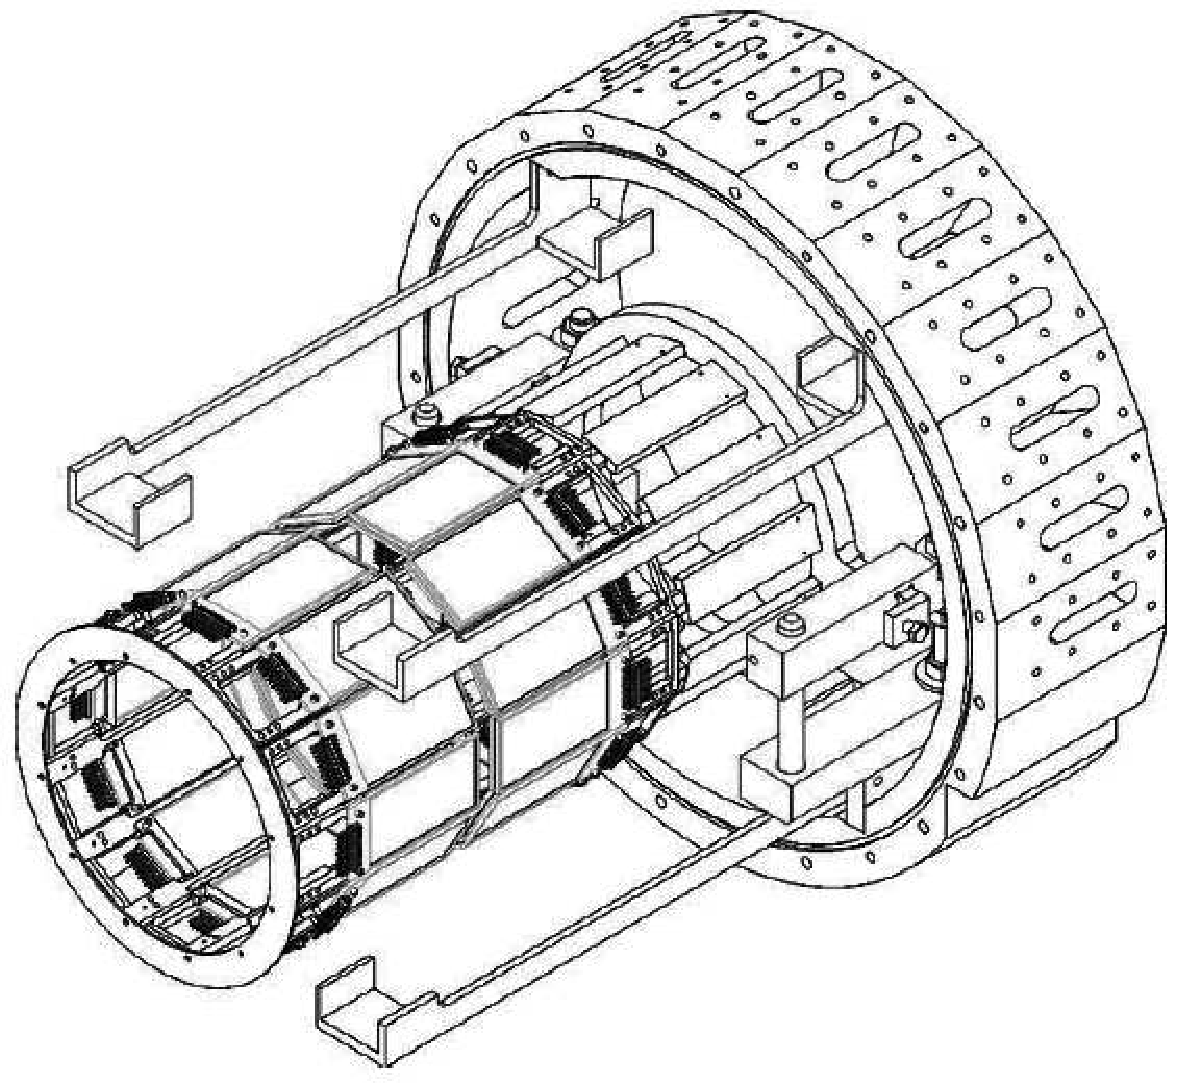
\includegraphics[width=\columnwidth,height=0.33\textheight,keepaspectratio]{Pain_2007-fig2}%
\caption[Engineering schematic of the ORRUBA detector system]{Engineering schematic of the ORRUBA detector system.  Beam enters from left.  In addition to showing two rings of detectors separated by a small gap, this figure also includes cable trays, the detector support structure and the preamplifier feedthrough ring.  Figure enhanced from Ref.~\cite{Pain_2007}.}%
\label{orruba}%
\end{figure}

The ORRUBA detector array, shown in Fig.~\ref{orruba}, is specifically designed to meet the challenges of measuring inverse kinematics: it has a large spacial coverage and is capable of making high resolution measurements of both energy and angle.  The details of the detector array construction are discussed in Ref.~\cite{Pain_2007}.  The ORRUBA detector array essentially consists of two rings of detectors positioned forwards and  backwards of $\theta_\mathrm{lab}=90^\circ$.  For the d($^{132}$Sn,p)$^{133}$Sn measurement, the upstream ring of detectors consisted of single-layer position sensitive detectors; the downstream ring was made up of $\Delta E$-$E$ telescopes, with the residual $E$ detectors also being position sensitive.  In this configuration, the detector array provides angular resolution of $<0.5^\circ$, position resolution of 0.5\,mm~FWHM, and (intrinsic) energy resolution of $<60$\,keV~FWHM.  Fig.~\ref{133Sn_e_spec_sim} shows a simulated spectrum of the d($^{132}$Sn,p)$^{133}$Sn based on these parameters.  The results of the simulation are in agreement with the analytic calculations of Fig.~\ref{sn-plots}.

\begin{figure*}
\begin{center}
\centering
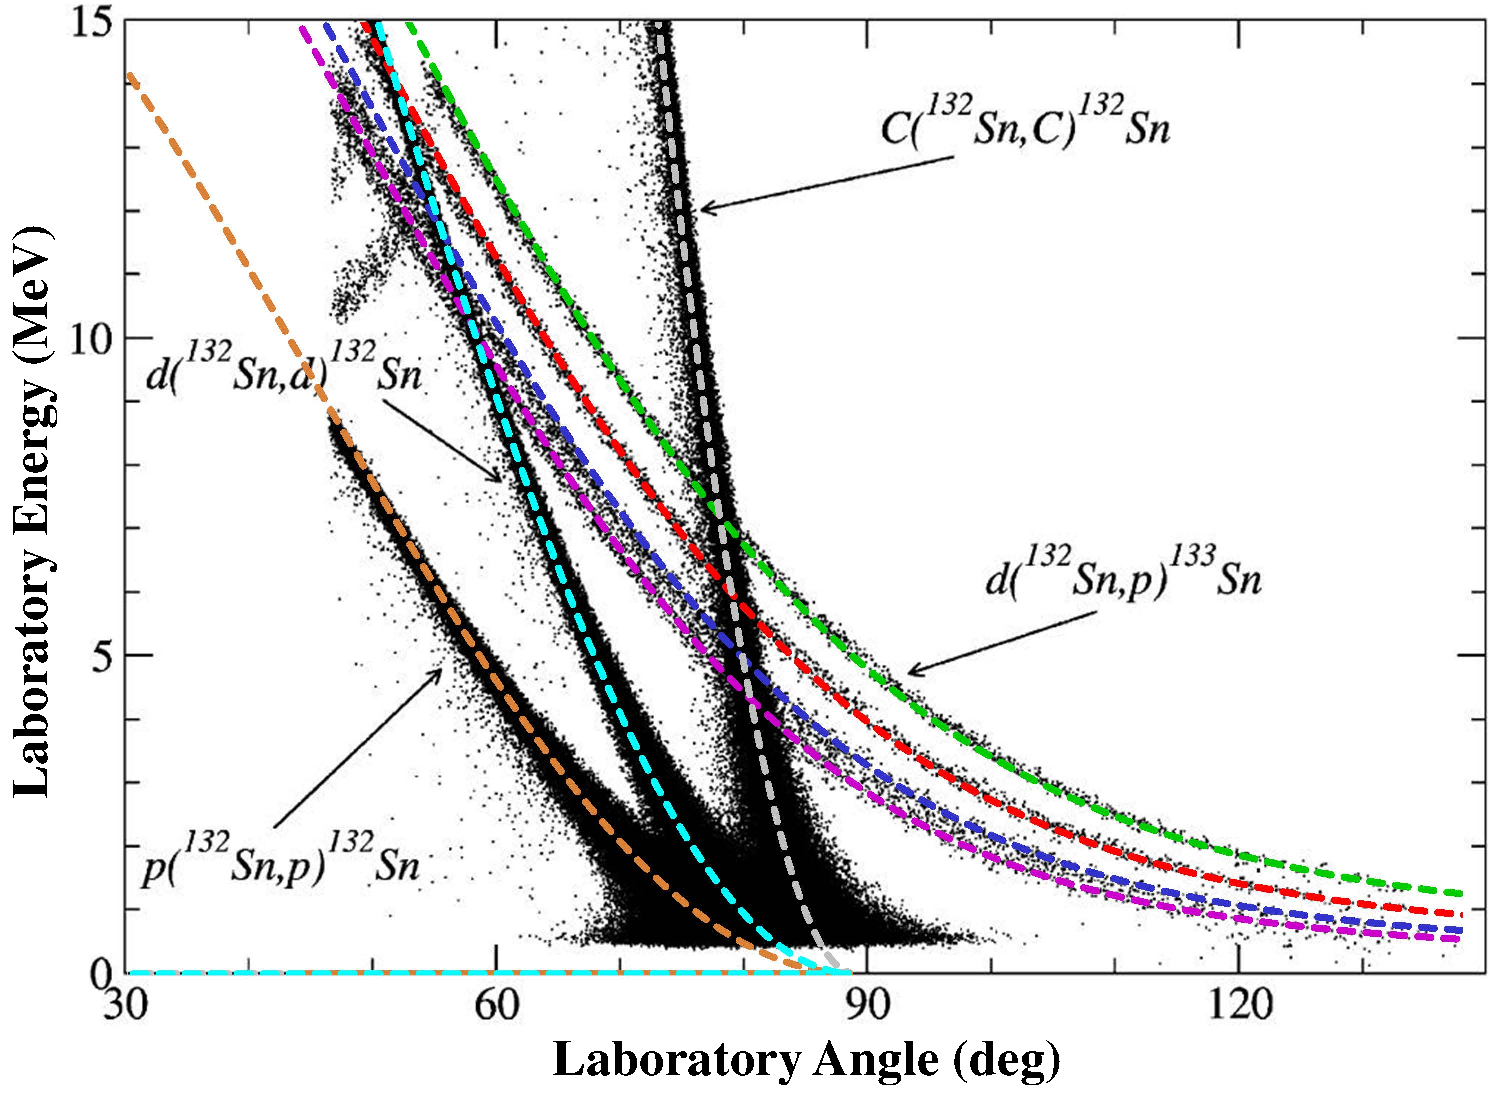
\includegraphics[keepaspectratio,height=0.3\textheight]{Pain_2007-fig1an-6}
\end{center}
\caption[Simulated $E_\mathrm{lab}$ vs. $\theta_\mathrm{lab}$ spectrum for the $d$($^{132}$Sn,$p$)$^{133}$Sn  reaction at 4.78\,\AMeV with ORRUBA]{(color online) Simulated $E_\mathrm{lab}$ vs. $\theta_\mathrm{lab}$ spectrum for the $d$($^{132}$Sn,$p$)$^{133}$Sn reaction at 4.78\,\AMeV with ORRUBA. The simulation includes elastic scattering of protons, deuterons, and $^{12}$C.  Analytical calculations have been plotted over the simulated results using the axes of the original figure.  The calculations are color-coded to match Fig.~\ref{133Sn_e}.  At $\theta_\mathrm{lab}=120^\circ$ 
  ($\theta_\mathrm{cm}=22.9^\circ$) the kinematic compression coefficient  is $\Delta E_\mathrm{lab}/\Delta E_\mathrm{cm}=0.34$.  Annotated    figure taken from Ref.~\cite{Pain_2007}.}
\label{133Sn_e_spec_sim}%
\end{figure*}

\subsection{Results}
\label{orrubaresults}
The ground-state and three excited states at $E_x=0.845$, 1.363, and 2005\,MeV were identified in this measurement. The state at $E_x=1.363\pm0.031$\,MeV was previously unobserved.  The $E_\mathrm{lab}$ versus $\theta_\mathrm{lab}$ proton spectrum produced is shown in Fig.~\ref{133Sn_e_spec}.  The analytic calculations of Fig.~\ref{sn-plots} have been plotted over the data (with re-calculated excitation energies).  Table~\ref{error_prop} shows that, neglecting target thickness effects, the $Q$-value resolution should be, at best, 133\,keV~FWHM.  Fig.~\ref{133Sn_e} shows the measured $Q$-value spectrum which has an energy resolution of over 300\,keV~FWHM.  Angular distributions were measured for the two lowest levels.  The ground state showed $\ell_n=3$ character, consistent with the $2f_{7/2}$ assignment; and the first-excited state at $E_x=0.845$ had an angular distribution characteristic of an $\ell_n=1$ transfer, corresponding to the $3p_{3/2}$ orbital.

\begin{figure*}
\begin{center}
\centering
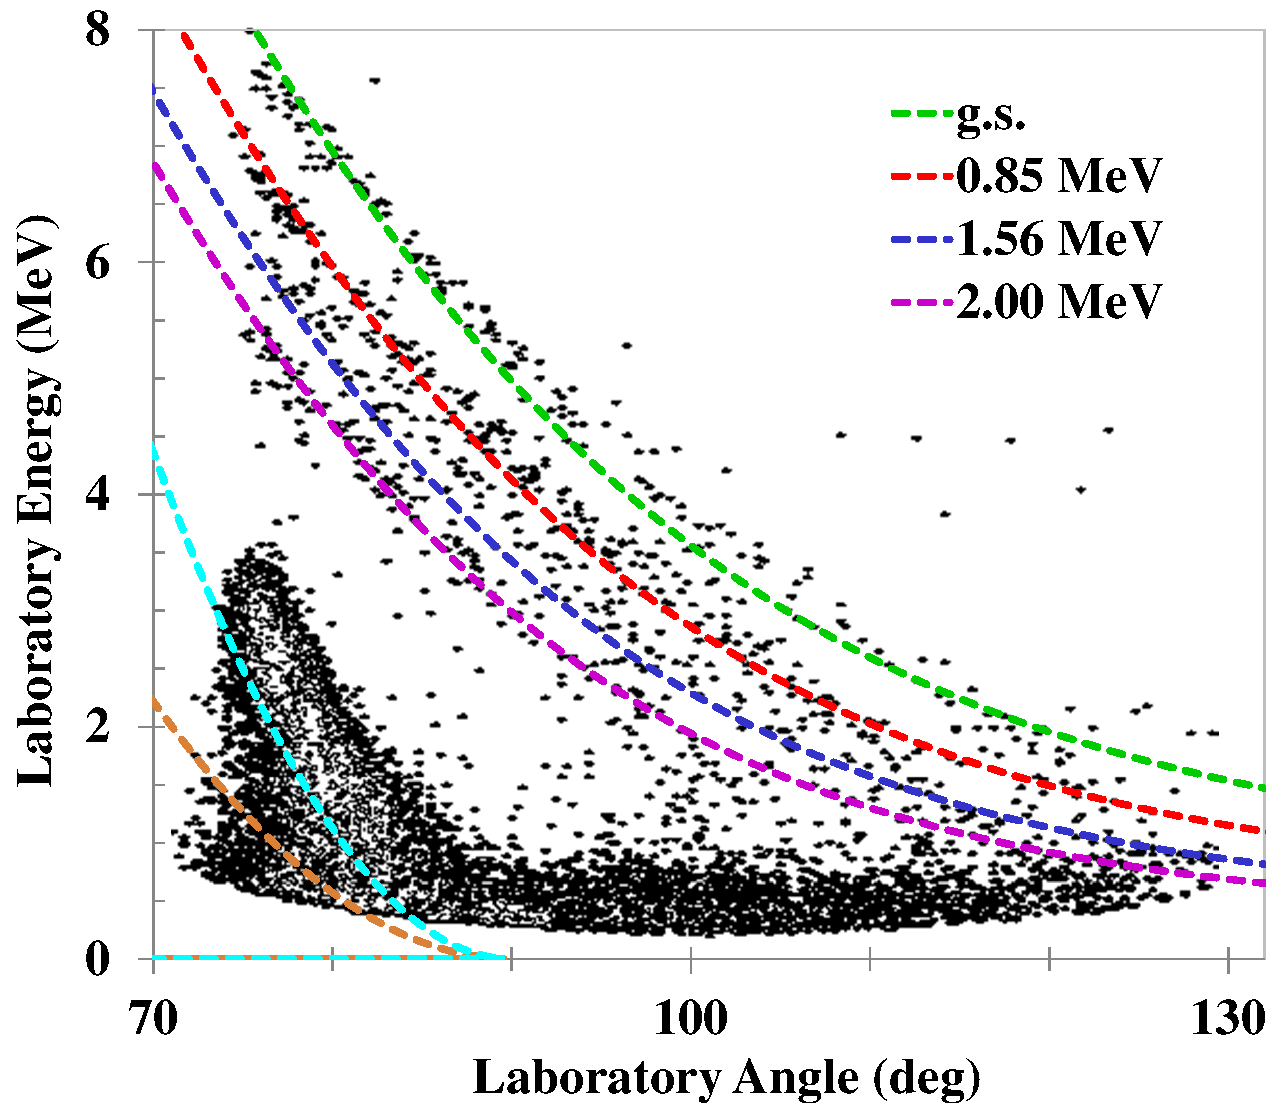
\includegraphics[keepaspectratio,height=0.3\textheight]{Jones_2007-2b}
\end{center}
\caption[Measured $E_\mathrm{lab}$ vs. $\theta_\mathrm{lab}$ spectrum for the $d$($^{132}$Sn,$p$)$^{133}$Sn reaction at 4.78\,\AMeV with ORRUBA]{(color online) Measured $E_\mathrm{lab}$ vs. $\theta_\mathrm{lab}$ spectrum for the $d$($^{132}$Sn,$p$)$^{133}$Sn reaction at 4.78\,\AMeV with ORRUBA.   Analytical calculations have been (roughly) plotted over the results, showing good agreement.  The axes of the calculations plot are shown.  Annotated figure taken from Ref.~\cite{Jones_2007}.}%
\label{133Sn_e_spec}%
\end{figure*}
%\subsection{Discussion}
Other reports are available in the literature of neutron transfer reactions in the $A=130$ region using ORRUBA.  An early proof-of-concept experiment was carried out using the lampshade SIDAR array and a prototypical form of the ORRUBA array to study the $^{124}$Sn($d$,$p$) reaction in inverse kinematics~\cite{Jones_2004}.  This measurement had a reported $Q$-value resolution of 200\,keV~FWHM.  %Using this set-up, the study was successful in producing a center-of-mass energy spectrum and the associated angular distributions.  Since then, 
Additional ($d$,$p$) studies have been carried out using %a more-complete form of 
the ORRUBA detector and other neutron-rich isotopes---$^{131}$Sn~\cite{Kozub_2008} and $^{134}$Te~\cite{Pain_2008}---both have excitation energy spectra with resolution on the order of 200--300\,keV~FWHM.  This collection of results provide a consistent description of the performance characteristics of this detector array.  In order to improve on the results obtained with ORRUBA, a detector system is needed which can avoid or suppress the effects of resolution degradation due to the covariance of measured quantities (kinematic broadening).

\begin{figure}[hb!]
\begin{center}
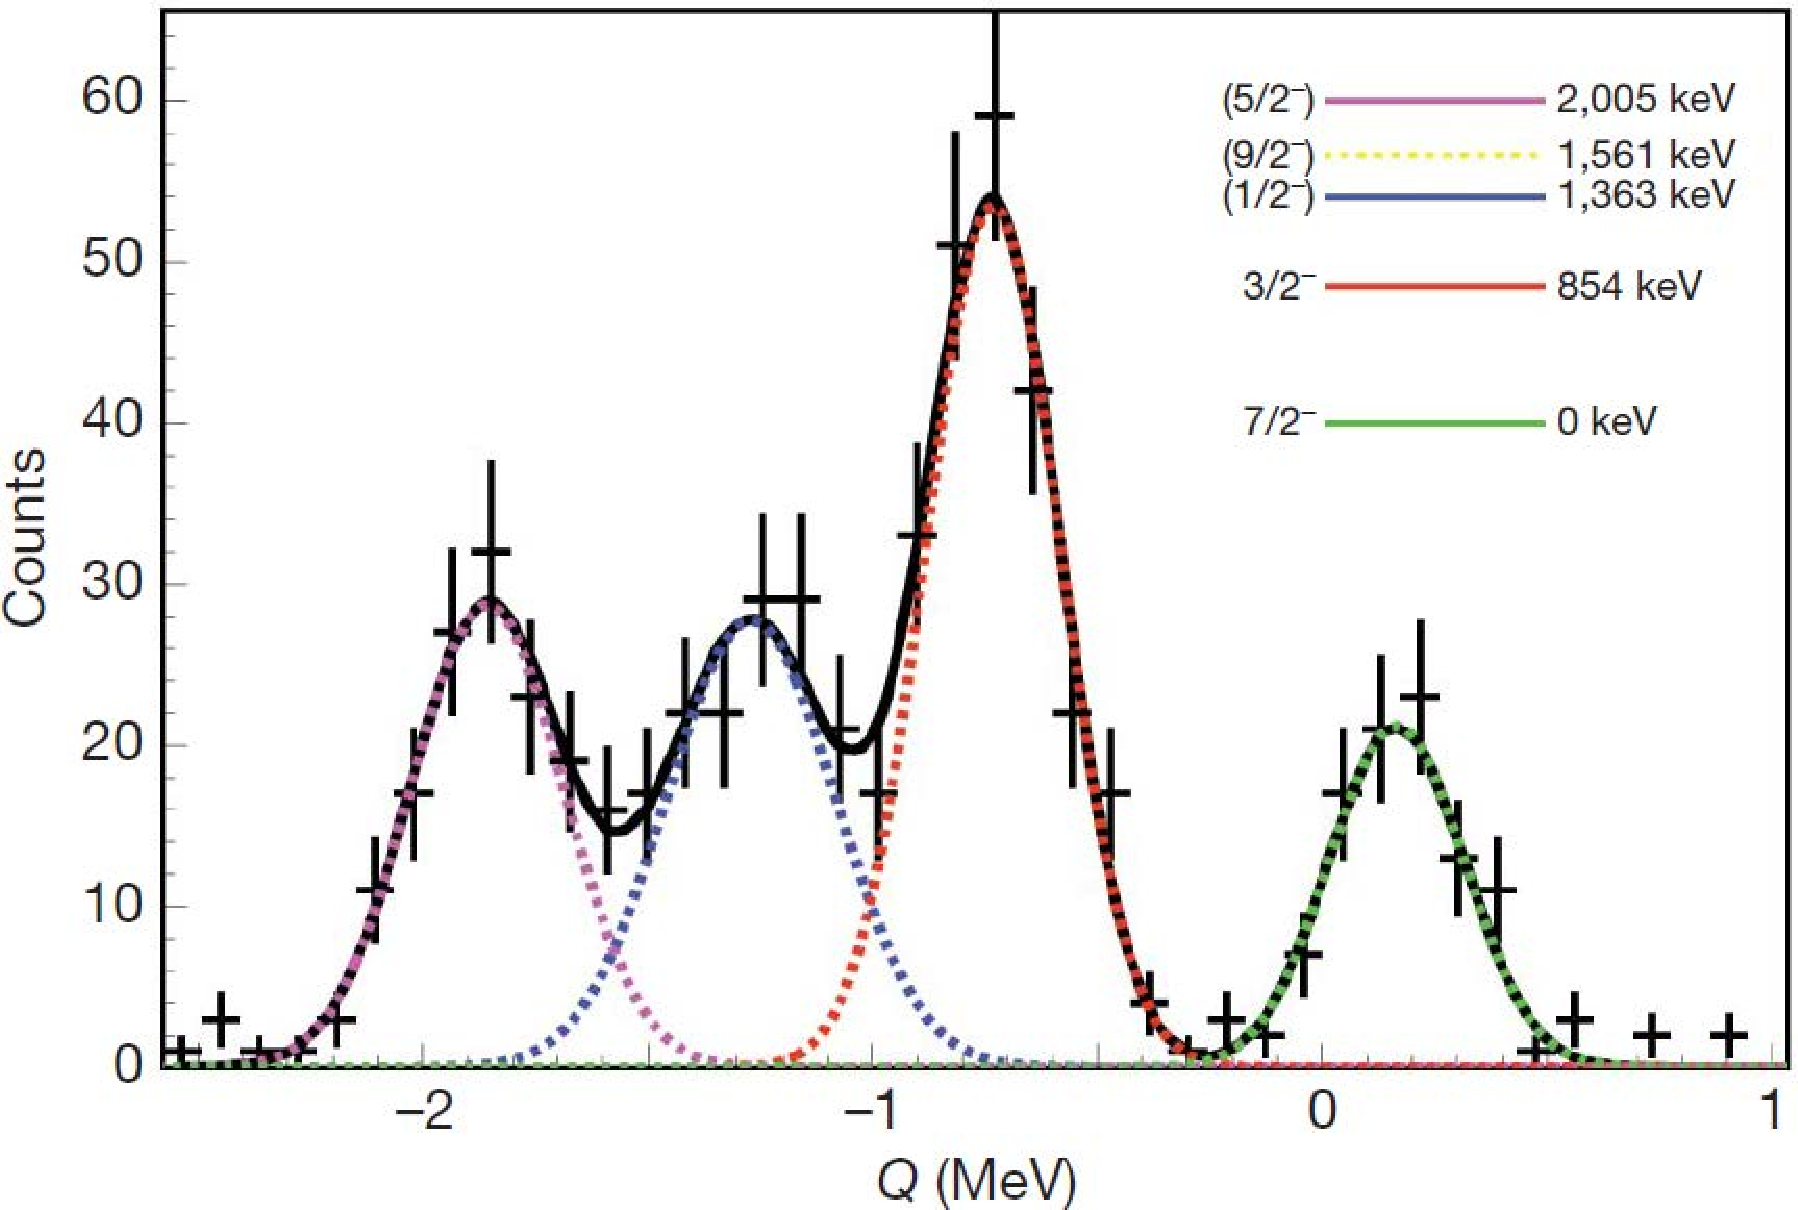
\includegraphics[keepaspectratio,width=\columnwidth,height=0.3\textheight]{Jones_2010-fig2-j}
\end{center}
\caption[$Q$-value spectrum from the $d$($^{132}$Sn,$p$)$^{133}$Sn reaction at 4.78\,\AMeV with ORRUBA]{(color online) $Q$-value spectrum from the $d$($^{132}$Sn,$p$)$^{133}$Sn reaction at 4.78\,\AMeV with ORRUBA.  Measured at $\theta_\mathrm{cm}=54^\circ$.  The $Q$-value resolution is 300\,keV~FWHM.  Figure taken from Ref.~\cite{Jones_2010}.}%
\label{133Sn_e}%
\end{figure}